\documentclass[final]{beamer}

% --- Packages ---
\usepackage[T1]{fontenc}
\usepackage{lmodern}
\usepackage[size=custom,width=91.44,height=121.92,scale=1.4]{beamerposter} 
\usepackage[utf8]{inputenc}
\usepackage{graphicx}
\usepackage{booktabs}
\usepackage{tcolorbox} 

% --- Color Definitions ---
\definecolor{siesgreen}{RGB}{46, 139, 87}
\definecolor{headerblue}{RGB}{0, 128, 128}

% --- Poster Setup ---
\setbeamertemplate{navigation symbols}{} 

% --- Global TColorBox Styles for Consistency ---
\tcbset{
    colbacktitle=headerblue,
    coltitle=black,
    fonttitle=\bfseries\huge,
    center title,
    left=12mm,   % Added internal padding to keep text away from sides
    right=12mm,
    top=10mm,
    bottom=10mm,
    boxrule=1mm  % Clean border thickness
}

\begin{document}
\begin{frame}[t]

% --- Header Section ---
\begin{tcolorbox}[colback=white, colframe=white, center, width=\textwidth, left=0mm, right=0mm]
    \centering
    \begin{columns}
        \column{0.2\textwidth}
        
\includegraphics[width=1.1\textwidth]{sies_gst_logonew.jpg} 
        
        \column{0.6\textwidth}
        \centering
        {\Huge \textbf{SIES Graduate School of Technology}} \\
        {\huge \textbf{AIML Department}} \\
        {\huge \textbf{2025-26}} \\
        \vspace{1cm}
        
    \end{columns}
    \begin{tcolorbox}[colback=siesgreen, colframe=black, arc=0mm, center, left=5mm, right=5mm]
            \centering \color{black} \Huge \textbf{NeuroLearn: BCI-Powered Adaptive Learning for Neurodiverse Individuals}
    \end{tcolorbox}
\end{tcolorbox}

\vspace{0.3cm}

% --- Main Content ---
\begin{columns}[t]

    % --- LEFT COLUMN ---
    \column{0.48\textwidth}
    
    \begin{tcolorbox}[title=ABSTRACT]
        \large Traditional “one-size-fits-all” education often fails to support neurodiverse learners. NeuroLearn addresses this by integrating Brain–Computer Interface (BCI) technology with intelligent learning systems. Using non-invasive EEG sensors, the system monitors learners’ real-time brain activity to estimate attention levels. The EEG data is analyzed using AI-driven algorithms to detect drops in focus and provides adaptive interventions—such as adjusting content difficulty—to re-engage learners.
    \end{tcolorbox}

    \vspace{0.3cm}

    \begin{tcolorbox}[title=INTRODUCTION]
        \large 
        \begin{itemize}
            \item Traditional education systems assume all students learn in the same way and at the same pace. However, neurodiverse students often have different learning styles and attention patterns. A rigid structure can limit their success; therefore, inclusive approaches are vital to support diverse cognitive needs.
            \item Most digital platforms measure engagement through behavioral data like clicks or time spent. These metrics do not truly reflect the attention or cognitive effort of a learner. Shifting toward tracking mental states—focus and cognitive load—enables truly personalized learning experiences.
        \end{itemize}
    \end{tcolorbox}

    \vspace{0.3cm}

    \begin{tcolorbox}[title=IMPACT AND BENEFITS]
        \large
        \begin{itemize}
            \item \textbf{Students:} Helps learners stay engaged by adapting content based on attention levels, enabling them to achieve their full academic potential.
            \item \textbf{Teachers:} Provides objective insights into student focus, helping educators identify challenges and tailor strategies to individual needs.
            \item \textbf{Society:} Promotes inclusive education aligned with National Education Policy (NEP) goals for personalized and equitable learning.
        \end{itemize}
    \end{tcolorbox}

    \vspace{0.3cm}

    \begin{tcolorbox}[title=FEASIBILITY \& BUDGET]
        \large The core hardware, including EEG sensors and microcontrollers, is commercially available and affordable, making low-cost prototypes highly viable for educational settings.
        \vspace{0.5cm}
        \centering
        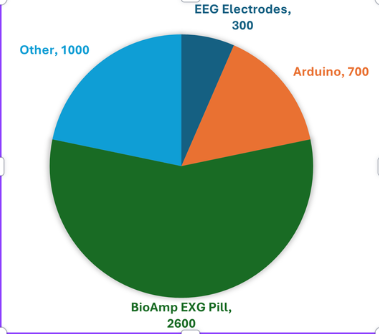
\includegraphics[width=0.6\textwidth]{budget_chart.png}
    \end{tcolorbox}

    % --- RIGHT COLUMN ---
    \column{0.48\textwidth}

    \begin{tcolorbox}[title=METHODOLOGY \& ARCHITECTURE]
        \centering
        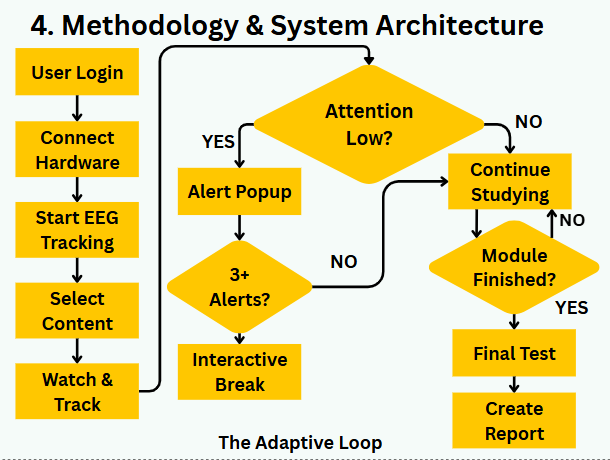
\includegraphics[width=0.8\textwidth]{flowchart.png}
        \vspace{0.5cm}
        \large
        \begin{itemize}
            \item \textbf{Monitor:} Non-invasive EEG sensors capture brain signals, amplified by the BioAmp EXG Pill. An Arduino UNO R4 digitizes this at 250 Hz, while webcams provide eye-tracking for added context.
            \item \textbf{Analyze:} The system uses ICA to remove noise like blinks. It calculates a "Focus Index" (Beta/Alpha ratio) and uses a 1D-CNN model to classify focus with up to 98\% accuracy.
            \item \textbf{Adapt:} Upon detecting distraction, the system pauses content and issues a focus alert. LLMs then generate interactive quizzes or simplified summaries to re-engage the learner.
        \end{itemize}
        \vspace{0.5cm}
        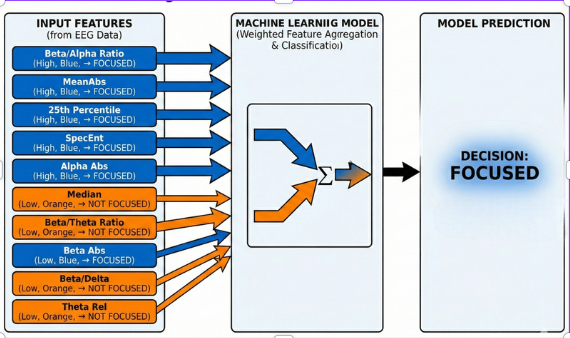
\includegraphics[width=0.8\textwidth]{xai.png}
    \end{tcolorbox}

    \vspace{0.3cm}

    \begin{tcolorbox}[title=CONCLUSION \& REFERENCES]
        \large NeuroLearner combines BCI with Generative AI to monitor attention and adapt learning in real time. This personalized, closed-loop system reduces cognitive overload and improves engagement for neurodiverse learners, turning frustration into academic success.
        
        \vspace{0.5cm}
        \begin{tcolorbox}[colback=white, colframe=black, left=5mm, right=5mm, top=5mm, bottom=5mm]
            \large % Increased size for group info
            \textbf{Group Members:} Mohit Paradkar, Nikhil Nair, Prem Rana, Tanmay Rewale \\
            \textbf{Guide:} Prof. Jasmin Hirani \\
            \textbf{Refs:} 1. braininformatics.springeropen.com | 2. link.springer.com
        \end{tcolorbox}
    \end{tcolorbox}

\end{columns}

\end{frame}
\end{document}